\documentclass{beamer}
\usetheme{Boadilla}

\usepackage[utf8]{inputenc}
\usepackage{tikz-cd}
\usepackage{wasysym}
\usepackage{physics}

\DeclareMathOperator{\Aut}{Aut}
\DeclareMathOperator{\Span}{span}

\title{KMS states and Tomita-Takesaki Theory}
\author[Iván Burbano]{Iván Mauricio Burbano Aldana\\[1cm]{\small Advised by: Prof. Andrés Fernando Reyes Lega}}
\institute{Universidad de los Andes}
\date{\today}

\begin{document}

\begin{frame}
	\titlepage
\end{frame}

\begin{frame}
	\frametitle{Motivation}
	\begin{columns}
		\column{0.5\textwidth}
		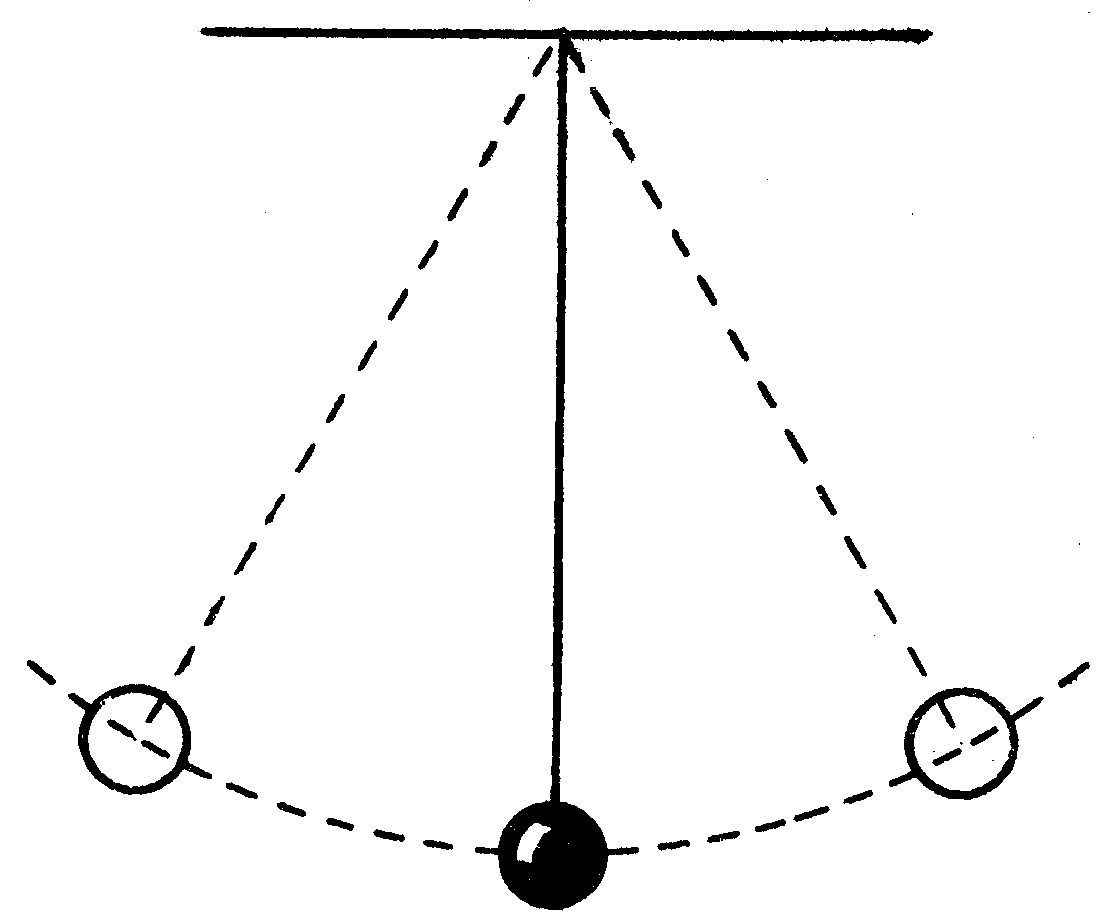
\includegraphics[width=\textwidth]{images/pendulum.png}
		\column{0.5\textwidth}
		Can we obtain the equations of motion from the equilibrium state?
		\vspace{1cm}
		
		\onslide<2->{Maybe in quantum thermal systems.
		\begin{align*}
			e^{-\beta H} &\circlearrowright e^{-iHt} \\
			\text{temperature} &\iff i\times\text{time}
		\end{align*}}
	\end{columns}
\end{frame}

\begin{frame}
	\frametitle{Outline}
	\tableofcontents
\end{frame}

\section{Classical and Quantum Theories}

\begin{frame}
	\frametitle{Elements of Classical and Quantum Theories}
	\begin{columns}
		\column{0.5\textwidth}
		Classical theories
		\begin{itemize}
			\item<1-> Auxiliary space: locally compact Hausdorff space $X$;
			\item<2-> Observables: continuous functions $C(X)$ on $X$;
			\item<3-> States: probability measures $P$ on $X$;
			\item<4-> Expected values: $\int fdP$.
		\end{itemize}
		\column{0.5\textwidth}
		Quantum theories
		\begin{itemize}
			\item<1-> Auxiliary space: separable Hilbert space $\mathcal{H}$
			\item<2-> Observables: self-adjoint operators on $\mathcal{H}$
			\item<3-> States: positive, self-adjoint, normalized and trace-class operators $\rho$ on $\mathcal{H}$;
			\item<4-> Expected values: $\tr(A\rho)$.
		\end{itemize}
	\end{columns}
\end{frame}

\begin{frame}[fragile]
	\frametitle{Difference between Classical and Quantum theories}
	\begin{equation*}
		\begin{tikzcd}
			\text{EPR paradox \cite{Einstein1935}} \arrow{d} \arrow{r} & \text{\onslide<2->{QM is incomplete}} \arrow{d} \\
			\text{\onslide<2->{QM is complete}} \arrow{d} & \begin{tabular}{c} \onslide<4->{Search for complete theory:} \\ \onslide<4->{Boolean propositions} \end{tabular} \arrow{d} \\
			\text{\onslide<3->{Entangled states \lightning}} \arrow{uur} & \begin{tabular}{c} \onslide<4->{Bell's inequalities  \cite{Bell1964}} \\ \onslide<4->{\cite{Reyes2013}} \end{tabular} \arrow{d} \\
			\text{\onslide<5->{Lattice of projections \cite{Wilce2012}}} & \text{\onslide<5->{Against experiment!}} \arrow{l}
		\end{tikzcd}
	\end{equation*}
\end{frame}

\section{Algebraic Quantum Mechanics}

\begin{frame}
	\frametitle{Algebraic Quantum Mechanics}
	\begin{itemize}
		\item Observables: A $C^*$-algebra $\mathcal{A}$:
		\begin{itemize}
			\item Complete normed vector space with product and involution;
			\item $C^*$ property: $\|A^*A\|=\|A\|^2$;
			\item A $C^*$-algebra can always be realized as a uniformly closed subset of the bounded operators on a Hilbert space\cite{Bratteli1987}. It is called a von Neumann algebra or $W^*$-algebra if $\mathcal{A}''=\mathcal{A}$ where the commutant $\mathfrak{A}'$ of a set $\mathfrak{A}$ of bounded operators on a Hilbert space is defined as the set of all bounded operatos which commute with every element of $\mathfrak{A}$.
			\item We will assume that all the algebras we discuss are unital.
		\end{itemize}
		\item States:  Linear functionals $\omega:\mathcal{A}\rightarrow\mathbb{C}$ which are non-negative ($\omega(A^*A)\geq 0$ and normalized ($\omega(1)=1$).
	\end{itemize}
\end{frame}

\begin{frame}
	\frametitle{GNS Construction}
	Start with a $C^*$-algebra $\mathcal{A}$ and a state $\omega$.
	\begin{itemize}
		\item $\mathcal{N}_\omega:=\{A\in\mathcal{A}|\omega(A^*A)=0\}$
		\item Hilbert space $\mathcal{H}_\omega := \overline{\mathcal{A}/\mathcal{N}_\omega}$ with $\langle [A], [B]\rangle := \omega(A^*B)$ 
		\item Define the representation extending
		\begin{alignat*}{2}
			\pi_\omega:\mathcal{A} & \rightarrow &\mathcal{B}(\mathcal{H}_\omega) \\
			A & \mapsto & \pi_\omega(A):\mathcal{H}_\omega & \rightarrow\mathcal{H}_\omega \\
			&& [B] & \mapsto [AB]
		\end{alignat*}
		\item Cyclic vector $\Omega_\omega := [1]$, that is, $\overline{\mathcal{A}\Omega_\omega}=\mathcal{H}_\omega$
		\item This is the unique $*$-representation of $\mathcal{A}$ with a cyclic vector $\Omega_\omega$ such that $\omega(A)=\langle\Omega_\omega,\pi_\omega(A)\Omega_\omega\rangle=\tr(\pi_\omega(A)\rho_{\Omega_\omega})$.
	\end{itemize}
\end{frame}

\begin{frame}
	\frametitle{Example: $M_{2\times 2}(\mathbb{C})$}
	Consider the most general state on this algebra
	\begin{equation}
		\omega_\lambda(A)=\lambda A_{11} + (1-\lambda) A_{22}=\tr(\rho_\lambda A),\quad\rho=\mqty[\lambda & 0\\0& 1-\lambda]
	\end{equation}
	for $\lambda\in[0,1]$. Let $E_{ij}$ be the matrix units so that $A=A_{ij}E_{ij}$
	\begin{equation*}
		\omega_\lambda(A^*A)=\omega_\lambda(A^*_{ki}A_{kj}E_{ij})=\lambda(|A_{11}|^2+|A_{21}|^2)+(1-\lambda)(|A_{12}|^2+|A_{22}|^2).
	\end{equation*}
	Therefore
	\begin{equation*}
		\mathcal{N}_\lambda=\begin{cases}
		\Span\{E_{11},E_{21}\} & \lambda = 0\\
		\Span\{E_{12},E_{22}\} & \lambda = 1\\
		\{0\} & \lambda\in(0,1)
		\end{cases}\quad
		\mathcal{H}_\lambda=\begin{cases}
		\Span\{E_{12},E_{22}\} & \lambda = 0\\
		\Span\{E_{11},E_{21}\} & \lambda = 1\\
		M_{2\times 2}(\mathbb{C}) & \lambda\in(0,1).
		\end{cases}
	\end{equation*}
\end{frame}

\begin{frame}
	\frametitle{Inner product}
	Consider $\lambda\in(0,1)$. We have for $e_{ij}=[E_{ij}]$, $\lambda_1:=\lambda$, and $\lambda_2:=1-\lambda$
	\begin{align}
	\begin{split}
		\langle e_{ij},e_{kl}\rangle=\omega(E_{ij}^*E_{kl})=\omega(E_{ji}E_{kl})=\omega(\delta_{ik}E_{jl})=\delta_{ik}\delta{jl}\lambda_l
	\end{split}
	\end{align}
	Therefore the basis $\{e_i^{(\alpha)}:=[E_{i\alpha}]/\sqrt{\lambda_\alpha}|i,\alpha\in\{1,2\}\}$ is an orthonormal basis for $\mathcal{H}_\lambda$. Moreover, the representation splits as
	\begin{equation}
		\mathcal{H}_\lambda=\mathcal{H}_\lambda^{(1)}\oplus\mathcal{H}_\lambda^{(2)}
	\end{equation}
	where $\mathcal{H}_\lambda^{(\alpha)}:=\Span\{e_i^{(\alpha)}|i\in\{1,2\}\}$. We have the corresponding orthogonal projections $P^{(\alpha)}$ onto $\mathcal{H}_\lambda^{(\alpha)}$.
	Another useful inner product to compute is
	\begin{equation}
		\langle\Omega_\lambda,e_i^{(\alpha)}\rangle=\frac{1}{\sqrt{\lambda_\alpha}}\langle[I_2],[E_{i\alpha}]\rangle=\frac{1}{\sqrt{\lambda_\alpha}}\omega(E_{i\alpha})=\frac{1}{\sqrt{\lambda_\alpha}}\delta_{i\alpha}\lambda_\alpha.
	\end{equation}
\end{frame}

\begin{frame}
	\frametitle{Constructing a Density Operator from Decompositions}
	\begin{align}
	\begin{split}
		\omega_\lambda(A)=&\langle\Omega_\lambda,\pi_\omega(A)\Omega_\omega\rangle=\langle\Omega_\omega,\sum_{\alpha\in I}P^{(\alpha)}\pi_\omega(A)\Omega_\omega\rangle\\
		=&\langle\Omega_\omega,\sum_{\alpha\in I}P^{(\alpha)}\pi_\omega(A)P^{(\alpha)}\Omega_\omega\rangle\\
		=&\langle\Omega_\omega,\sum_{n\in J}\langle e_n,\sum_{\alpha\in I}P^{(\alpha)}\pi_\omega(A)P^{(\alpha)}\Omega_\omega\rangle e_n\rangle\\
		=&\sum_{n\in J}\langle e_n,\sum_{\alpha\in I}P^{(\alpha)}\pi_\omega(A)P^{(\alpha)}\langle\Omega_\omega,e_n\rangle\Omega_\omega\rangle\\
		=&\sum_{n\in J}\langle e_n,\sum_{\alpha\in I}P^{(\alpha)}\pi_\omega(A)P^{(\alpha)}\rho_{\Omega_\omega}e_n\rangle\\
		=&\tr(\pi_\omega(A)\sum_{\alpha\in I}P^{(\alpha)}\rho_{\Omega_\omega}P^{(\alpha)})=\tr(\pi_\omega(A)\rho_\omega)
	\end{split}
	\end{align}
\end{frame}

\begin{frame}
	\frametitle{The Density Operator of Our Decomposition}
	\begin{align}
	\begin{split}
		\rho_\lambda e_i^{\alpha}=&\sum_{\beta\in I}P^{(\beta)}\rho_{\Omega_\omega}P^{(\beta)}e_i^{(\alpha)}=\sum_{\beta\in I}P^{(\beta)}\rho_{\Omega_\omega}\delta_{\alpha\beta}e_i^{(\alpha)}=P^{(\alpha)}\rho_{\Omega_\omega}e_i^{(\alpha)}\\
		=&P^{(\alpha)}\frac{1}{\sqrt{\lambda_\alpha}}\delta_{i\alpha}\lambda_\alpha\Omega_\omega=\frac{1}{\sqrt{\lambda_\alpha}}\delta_{i\alpha}\lambda_\alpha\sum_{j=1}^2\langle e_j^{\alpha},\Omega_\omega\rangle e_j^{(\alpha)}\\
		=&\frac{1}{\sqrt{\lambda_\alpha}}\delta_{i\alpha}\lambda_\alpha\sum_{j=1}^2\frac{1}{\sqrt{\lambda_\alpha}}\delta_{j\alpha}\lambda_\alpha e_j^{(\alpha)}=\frac{1}{\sqrt{\lambda_\alpha}}\delta_{i\alpha}\lambda_\alpha\frac{1}{\sqrt{\lambda_\alpha}}\lambda_\alpha e_\alpha^{(\alpha)}\\
		=&\delta_{i\alpha}\lambda_\alpha e_\alpha^{(\alpha)}.
	\end{split}
	\end{align}
	Therefore, in the ordered basis $\mathcal{B}=\{e_1^{(1)},e_2^{(1)},e_1^{(2)},e_2^{(2)}\}$ we have
	\begin{equation}
		[\rho_\lambda]_\mathcal{B}=\mqty[\lambda & 0 & 0 & 0\\ 0 & 0 & 0&0\\0&0&0&0\\0&0&0&\sqrt{1-\lambda}]
	\end{equation}
\end{frame}

\begin{frame}
	\frametitle{The representation}
	Finally we explicitly need the GNS representatives. Using the same approach
	\begin{equation*}
		\pi_\lambda(A)e_i^{(\alpha)}=\frac{1}{\sqrt{\lambda_\alpha}}[AE_{i\alpha}]=\frac{1}{\sqrt{\lambda_\alpha}}[A_{jk}\delta_{ki}\delta_{\beta\alpha}E_{j\beta}]=\frac{1}{\sqrt{\lambda_\alpha}}A_{ji}[E_{j\alpha}]=A_{ji}e_j^{(\alpha)}.
	\end{equation*}
	Therefore
	\begin{equation}
		[\pi_\lambda(A)]_\mathcal{B}=\mqty[A & 0\\0 &  A]
	\end{equation}
	and we explicitly check that neither $\rho_{\Omega_\lambda}$ or $\rho_\lambda$ have an interpretation as observables.
\end{frame}

\begin{frame}
	\frametitle{Ambiguity in functions of states}
	Consider the von Neumann entropy $S(\rho)=-\tr(\rho\log(\rho))$ of a density matrix $\rho$. In our example the entropy of our initial density matrix describing the state is $-\lambda\log(\lambda)-(1-\lambda)\log(1-\lambda)=S(\rho)=\omega(\log(\rho))$. This is in particular the expected value of an observable! However, in the GNS representation we have encountered two density matrices which also do the job $\rho_{\Omega_\lambda}$ and $\rho_\lambda$ but are not observables. The first has a null entropy since it is a vector state $S(\rho_{\Omega_\lambda})=0$. On the other hand $S(\rho_\lambda)=S(\rho)$. What is going on here? In reality, the ambiguity is much more dramatic. Redefining the orthonormal basis by $e_i^{\alpha}(U)=\sum_\beta=1^2e_i^{(\beta)}U_{\beta\alpha}$ for $U$ unitary yields a new decomposition and thus a new density operator $\rho_\lambda(U)$. More about this will be discussed in Souad's lecture right after this!
\end{frame}

\begin{frame}
\frametitle{Cyclic representations of $W^*$-algebras}
\begin{theorem}[$\bigstar$]
If $\mathfrak{M}$ is a $W^*$-algebra and $\omega$ is a faithful ($\omega(A^*A)=0\rightarrow A=0$) normal ($\omega(A)=\tr(\rho A)$) state then its cyclic representation $(\mathcal{H}_\omega,\pi_\omega,\Omega_\omega)$ satisfies
\begin{itemize}
	\item $\pi_\omega$ is faithful (injective);
	\item $\pi_\omega(\mathfrak{M})$ is a von Neumann algebra;
	\item $\Omega_\omega$ is separating for $\pi_\omega(\mathfrak{M})$ ($\pi_\omega(A)\Omega_\omega=0\rightarrow\pi_\omega(A)=0$).
\end{itemize}
\end{theorem}
\end{frame}

\begin{frame}
	\frametitle{Dynamical Systems}
	Time evolution is represented by a one-parameter group of automorphisms
	\begin{align*}
		\tau:\mathbb{R}&\rightarrow\Aut(\mathcal{A}) \\
		t&\mapsto\tau_t.
	\end{align*}
	Dynamical systems consist of an $C(W)^*$-algebra with a time evolution which satisfies certain continuity properties.
	\begin{example}
	Given a Hamiltonian $H$ on a Hilbert space $\mathcal{H}$ the Schrödinger time evolution $s$ is given by
	\begin{equation}
	s_t(O)=e^{iHt}O e^{-iHt}
	\end{equation}
	and $(\mathcal{B}(\mathcal{H}),s)$ is a dynamical system.
	\end{example}
\end{frame}

\section{KMS States}

\begin{frame}
	\frametitle{KMS States}
	\begin{definition}
	Let $(\mathcal{A},\alpha)$ be a dynamical system. $\phi$ is said to be a KMS state if for all $A,B\in\mathcal{A}$ there exists an analytic $F$ on the strip which satisfies
	\begin{figure}
		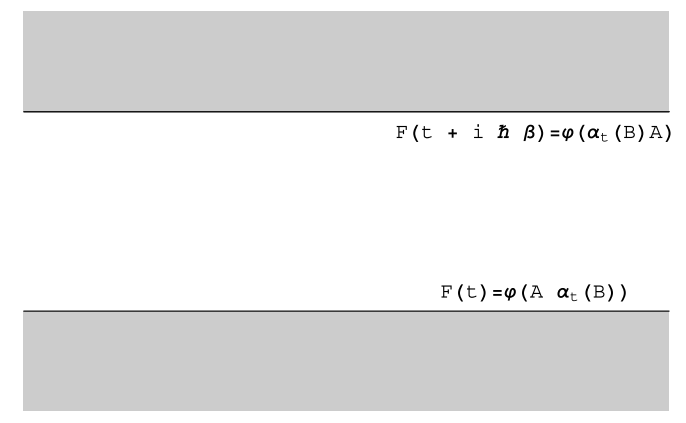
\includegraphics[width=0.6\textwidth]{images/kms.png}
		\caption{Taken from \cite{Connes1994}.}
	\end{figure}
	\end{definition}
\end{frame}

\begin{frame}
	\frametitle{KMS states as Equilibrium states}	
	KMS states are a candidate for a general definition of thermodynamic equilibrium in quantum systems\cite{Haag1967}:
	\begin{itemize}
		\item KMS states are invariant under the dynamics $\omega(\tau_t(A))=\omega(A)$;
		\item In finite dimensional Hilbert spaces with Schrödinger's time evolution $\tau$, the only possible $(\tau,\beta)$-KMS states are the $\beta$-Gibbs states
		\begin{align*}
			\mathcal{B}(\mathcal{H})&\rightarrow\mathbb{C} \\
			A&\mapsto \frac{\tr(Ae^{-\beta H})}{\tr(e^{-\beta H})}.
		\end{align*}
		\item It is clear that the Gibbs prescription cannot be the characterization of equilibrium in the thermodynamic limit since coexistence of different phases demands that there cannot be a general unique correspondence between the Hamiltonian (evolution group) and states\cite{Connes1994}.
	\end{itemize}
\end{frame}

\section{Tomita-Takesaki Theory}

\begin{frame}
	\frametitle{Tomita-Takesaki Theory}
	For a $W^*$-algebra $\mathfrak{M}$ equipped with a cyclic and separating vector $\Omega$ Tomita-Takesaki theory yields:
	\begin{itemize}
		\item a one-parameter unitary group $t\mapsto\Delta^{it}$;
		\item a modular conjugation $J$.
	\end{itemize}
	\begin{theorem}[Tomita-Takesaki]
		\begin{itemize}
			\item $J\mathfrak{M}J=\mathfrak{M}'$;
			\item $\Delta^{it}\mathfrak{M}\Delta^{-it}=\mathfrak{M}$ for all $t\in\mathbb{R}$. 	
		\end{itemize}
	\end{theorem}
	\begin{proof}
		\cite{Bratteli1987}
	\end{proof}
\end{frame}

\begin{frame}
	\frametitle{Modular Automorphism Group}
	\begin{definition}
		Let $\mathfrak{M}$ be a von Neumann algebra and $\omega$ be a faithful normal state. Due to $\bigstar$ we can perform the modular constructions on the cyclic representation $(\pi_\omega(\mathfrak{M}),\pi_\omega,\Omega_\omega)$. We define the modular automorphism group of $(\mathfrak{M},\omega)$ by 
		\begin{equation}
			\alpha_t=\pi_\omega^{-1}(\Delta^{it}\pi_\omega(A)\Delta^{-it}).
		\end{equation}
	\end{definition}
	\begin{theorem}[$\bigstar\bigstar$]
		$(\mathfrak{M},\alpha)$ is a $W^*$-dynamical system  
	\end{theorem}		
	\begin{proof}
		\cite{Duvenhage1999}
	\end{proof}
\end{frame}

\section{The Canonical Time Evolution}

\begin{frame}
	\frametitle{The Canonical Time Evolution}
	\begin{theorem}[$\bigstar\bigstar\bigstar$]
		Let $\mathfrak{M}$ be a von Neumann algebra and $\omega$ be a faithful normal state. Then $(\mathfrak{M},\tau)$ with $\tau_t(A) = \alpha_{-t/\beta}(A)$ and $\alpha$ the modular group of $(\mathfrak{M},\omega)$ is the unique $W^*$-dynamical system such that $\omega$ is a $(\tau,\beta)$-KMS state.
	\end{theorem}
	\begin{proof}
		\cite{Duvenhage1999}
	\end{proof}
\end{frame}

\begin{frame}
	\frametitle{On von Neumann Algebras as Dynamical Objects}
	\begin{itemize}
		\item Through the modular group, states induce dynamics on the algebra of operators.
		\item The physical relevance of such prescription for evolution is guaranteed by the fact that it is the unique  dynamical law which makes the state an equilibrium state.
		\item One can use an analog of the Radon-Nikodym theorem to connect the modular groups induced by different states. Such a connection brings forward a canonical  homomorphism from $\mathbb{R}$ into the automorphism group of $\mathfrak{M}$ modulus inner automorphisms. This suggests that the emergence of the dynamical law might have a deeper origin.  
	\end{itemize}
\end{frame}

\begin{frame}[allowframebreaks]
	\frametitle{References}
	\bibliography{../Mendeley/library}
	\bibliographystyle{apalike}
\end{frame}

\end{document}